\chapter{Shifted periodic boundary conditions for simulations of wall-bounded turbulent flows}% Force line breaks with \\

\begin{abstract}
In wall-bounded turbulent flow simulations, periodic boundary conditions combined with insufficiently long domains lead to persistent spanwise locking of large-scale turbulent structures. This leads to statistical inhomogeneities of 10\% to 15\% that persist in time averages of 60 eddy turnover times and more. We propose a shifted periodic boundary condition that eliminates this effect without the need for excessive streamwise domain lengths. The method is tested based on a set of direct numerical simulations of a turbulent channel flow, and large-eddy simulations of a high Reynolds number rough-wall half-channel flow. The method is very useful for precursor simulations that generate inlet conditions for simulations that are spatially inhomogeneous, but require statistically homogeneous inlet boundary conditions in the spanwise direction. The method's advantages are illustrated for the simulation of a developing wind-farm boundary layer.
\end{abstract}


% % % % % % % % % % % % % % % % % % % % % % % % % % % % % % % % % % % % % % % % % %
\section{Introduction}\label{sec:intro}
% % % % % % % % % % % % % % % % % % % % % % % % % % % % % % % % % % % % % % % % % %

In turbulence-resolving simulation approaches such as direct numerical simulations (DNS) and large-eddy simulations (LES), periodic boundary conditions are often applied. They recycle turbulent fluctuations back into the domain, providing an efficient means to achieve fully-developed turbulent inflow conditions. This approach is mostly the method of choice for simulation of fully developed boundary layer flows, such as DNS of turbulent channel flows,\cite{kim1987turbulence} pipe flows,\cite{monty2007large,wu2008direct} Couette flows,\cite{takahiro2006dns} etc., and similar studies based on LES. Moreover, periodic boundary conditions are also often used for the generation of fully developed inflow turbulence for streamwise developing wall-bounded flows, using a so-called precursor simulation.\cite{tabor2010inlet, stevens2014concurrent}

When using periodic boundary conditions to generate fully developed turbulence, any nonphysical influence originating from the perfect correlations over the periodic domain length should be avoided. To this end, the size of the computational domain should be chosen to be several times larger than the largest scales in the flow. In boundary layers, experimental and numerical studies have shown the existence of very large streamwise-elongated coherent structures, with length scales of the order of tens of boundary layer thicknesses $\delta$ (see, e.g., Refs \cite{delalamo2003spectra, delalamo2004scaling, jimenez1998largest, tomkins2003spanwise, hutchins2007evidence, lu2010modulated, lozanoduran2014effect}). These structures are ubiquitous in neutral wall-bounded flows, ranging from lower Reynolds number laboratory-scale flows to the high Reynolds number atmospheric boundary layers (ABL).\cite{balakumar2007large,hutchins2012towards} In the literature, these streaky structures are commonly referred to as superstructures\cite{hutchins2007evidence} or Very-Large-Scale Motions (VLSM).\cite{kim1999very, fang2015large} As a consequence of these very long structures, domain lengths $L_x$ in streamwise periodic wall-bounded turbulent flow simulations may need to be on the order of $L_x=32\pi\delta$ to  $60\pi\delta$, in order to fully capture them.\cite{lozanoduran2014effect,fang2015large} 

At these domain lengths, simulations become very expensive, and lack of computational resources has often led to the use of domain sizes that are much smaller, e.g., $L_x=2\pi\delta$ is a choice often encountered in the literature. However at too short domain lengths, superstructures lack the streamwise space to significantly meander or break up before they are recycled back to the inlet. Thus, they become virtually infinitely long, and remain locked in time at the same spanwise position by the persistent recycling. Simulation results of spanwise-homogeneous flows in too short domains are therefore biased to have sustained streamwise-oriented bands of high and low speed velocity, even after very long time averaging (see, e.g., Refs \cite{finnigan2009turbulence, lu2010modulated, verhulst2014large, fang2015large, boppana2014thermal, alqadi2015large}). As, e.g., discussed by Lozano-Dur\'an \& Jim\'enez\cite{lozanoduran2014effect} these quasi-infinite structures in too short simulation domains do ``capture most of the effects of the actual structures, or at least of their interactions with smaller scales of size $\mathcal{O}(\delta)$.'' As a result, horizontally and time averaged profiles are not affected (as also shown in the current paper). However, this persistent spanwise inhomogeneity is very important in cases where the fully developed turbulence in a precursor simulation is used as an inlet boundary condition to a simulation which is not homogeneous in the spanwise direction. This phenomenon has also been investigated by Fishpool et al.\cite{fishpool2009persistent} for channel flows at $Re_\tau$ = 180 and 410, with streamwise domain lengths $L_x = 4\pi\delta$ and $2\pi\delta$ respectively. It was found that, in both flow cases, the locking effect led to significant spanwise variations in time-averaged velocity. In this paper, we propose a \emph{shifted periodic boundary condition} which, in contrast to classical periodic boundary conditions, adds a spanwise offset (i.e. shift) to the outflow plane before reintroduction at the inlet. 

The paper is structured as follows. Section \ref{sec:methodology} elaborates on the proposed shifted periodic boundary conditions. Section \ref{sec:wbturbflows} applies the method to both a channel flow DNS at $Re_\tau = 395$ and a very high Reynolds number half-channel flow LES with varying streamwise domain lengths, including a comparison with classical periodic boundary conditions for both cases. Section \ref{sec:windfarm} subsequently uses shifted periodic boundary conditions in a precursor simulation for a wind-farm LES, illustrating a possible use case for the method. Section \ref{sec:conclusion} finally provides a brief summary of the main conclusions and contributions of this work.

% % % % % % % % % % % % % % % % % % % % % % % % % % % % % % % % % % % % % % % % % % 
\section{Shifted periodic boundary conditions}\label{sec:methodology}
% % % % % % % % % % % % % % % % % % % % % % % % % % % % % % % % % % % % % % % % % % 

In the current paper, we propose a \emph{shifted periodic boundary condition} approach that prevents the spanwise locking of large-scale structures in simulation domains that are too short. The methodology is illustrated in Figure \ref{fig:concept}. Instead of straightforwardly reintroducing the velocity from the outlet plane back at the inlet, this plane is first shifted uniformly in the spanwise direction by a predefined and constant distance $d_s$. 

The shifting distance $d_s$ is the only user-defined parameter in the method. The main constraint for choosing $d_s$ is to avoid reintroduction of turbulent structures by the shifting operation at exactly the same spanwise location after only a limited number of flowthroughs. Since spanwise boundary conditions remain periodic, such a situation would occur after $N$ flowthroughs, where $N d_s = M L_y$ with $N$ and $M$ integers. Mathematically, this means that the ratio $L_y/d_s$, when expressed as a simple fraction of integers in its lowest terms, should have a large numerator. Equivalently, $d_s$ and $L_y$ should have a large least common multiple to assure a large $N$. This is illustrated graphically in Figure 2 for $d_s = \delta/2$ and $d_s = L_y/2$. The figure shows adjacent copies of velocity field planviews, shifted in the spanwise direction with the respective $d_s$ at the streamwise domain boundaries. The arrows illustrate where turbulent structures will be reintroduced after flowing through the domain. It can be observed from the figure that choosing $d_s = L_y/2$ results in structures arriving at the exact same spanwise location after only 2 flowthroughs.

In practice, we propose to choose $d_s$ such that it flattens out the spanwise variations as quickly as possible. 
Therefore, we choose a value of $d_s = 0.5\delta$ since this is roughly equal to the spanwise length-scale of the largest turbulent structures in the wall-bounded flows studied here. \cite{tomkins2003spanwise, hutchins2007evidence,fang2015large} 
In this way, the large-scale structures gradually sweep the spanwise extent of the domain. 
Note that this length-scale is dependent on factors such as Reynolds number and distance to the wall. 
Therefore, we verified that other values also yield satisfactory results (e.g. $d_s = \delta/4$, $\delta$, $3\delta/2$), provided that $d_s$ and $L_y$ have no ``small'' least common multiple.

The spanwise domain boundaries are still treated with standard periodic boundary conditions. This allows us to reconstruct a continuous inflow plane at the streamwise inflow boundary since, after shifting, the portion of the outflow plane which falls out of range can now be remapped to the other side, as shown by the dashed arrows and the indicated flow structure in Figure \ref{fig:concept}b. The methodology, although conceptually simple, leads to significant improvements in the spanwise homogeneity of time-averaged flow fields, as is shown below.

For standard numerical discretizations, e.g. by the finite-difference of finite-volume approach, the proposed shifted periodic boundary conditions can be straightforwardly imposed in a similar way as traditional periodic boundary conditions, albeit with a spanwise shift. However, in turbulent flow simulations,  spectral methods are often the method of choice due to their superior accuracy. This is also the case in the current paper, where we apply a Fourier pseudo-spectral discretization in the horizontal directions (see further below for a description of our solver). Note that this discretization requires true global periodicity, and is hence incompatible with a direct implementation of shifted periodic boundary conditions. This incompatibility is circumvented by the use of a fringe region technique: as shown in Figure \ref{fig:concept}c an auxiliary region is appended to the back side of the original simulation domain. At the end of the extended domain a fringe region is defined, in which the Navier-Stokes solution is smoothly nudged towards a spanwise-shifted version of the flow field at the original effective domain length $x = L_{\textit{\small x,eff}}$. This nudging is performed in every timestep through the addition of a body force term in the momentum equations. The smoothness of the latter averts the risk of both spuriously contaminating the computation of pressure throughout the domain and introducing oscillations in the velocity field. The outflow is then reintroduced at the domain inlet through the global periodic boundary conditions. The solid arrows in Figure \ref{fig:concept} summarize the flow of information as discussed above. Note that, in contrast to traditional periodic boundary conditions, in the current implementation there is no direct feedback from the flow field at the inlet of the domain (at $x=0$) to the flow field at the ``effective" outlet of the domain (at $x=L_{\textit{x,eff}}$). 

In the simulations discussed in the following sections, the Poisson equation for pressure is solved using a {\color{red} DFT}-based technique, hence the pressure field is also subjected to globally periodic boundary conditions. In case the currently proposed shifted boundary conditions are implemented in a standard flow solver, for which the Poisson equation requires appropriate pressure boundary conditions, the same spanwise-shifted periodic boundary conditions, as used for velocity, can be applied for pressure as well.


\begin{figure}[t]
	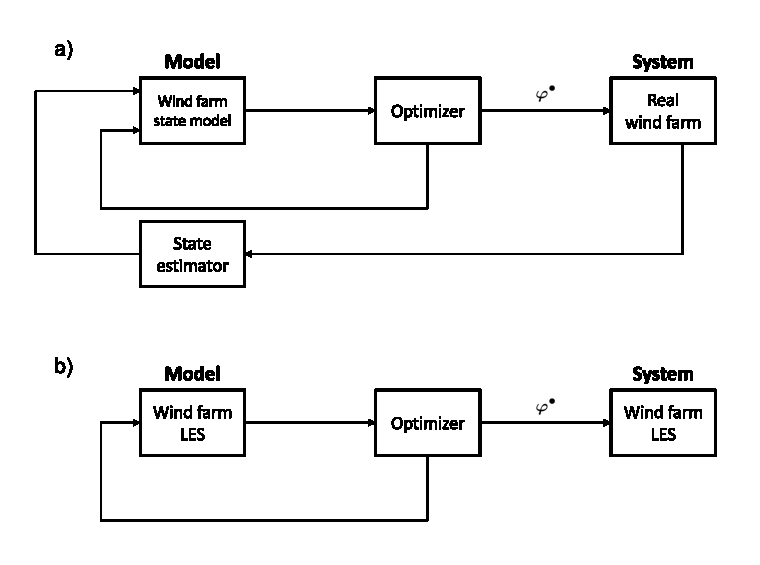
\includegraphics[width=\textwidth]{chapters/pof_shifting/figure1}
	\caption{Visualization of shifted periodic boundary condition concept for a turbulent half-channel simulation. The flow direction is indicated by the blue dashed arrows. \emph{a)} Classic periodic boundary conditions. \emph{b)} Shifted periodic boundary conditions, $d_s$ indicates shifting distance. Original (pre-shift) spanwise domain boundary indicated by black dot-dashed line in the inlet plane. The encircled structure illustrates how planes can be ``wrapped around'' the spanwise periodic boundary conditions. \emph{c)} Implementation in a solver with Fourier pseudo-spectral discretization in the streamwise direction, requiring global periodicity. The shaded region indicates the \emph{fringe} region.}
	\label{fig:concept}
\end{figure}

\begin{figure}[t]
	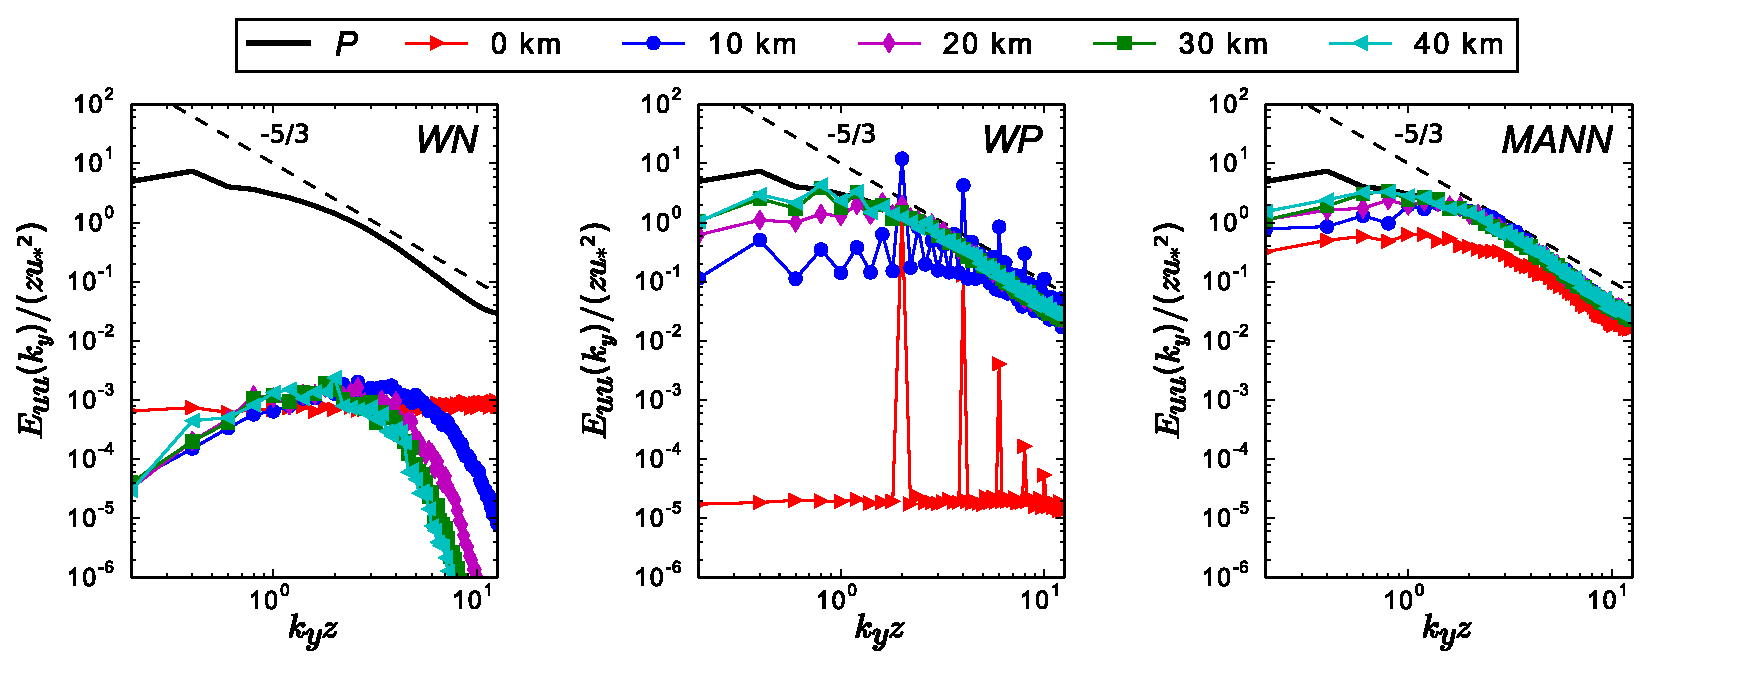
\includegraphics[width=0.7\textwidth]{chapters/pof_shifting/figure2}
	\caption{Spanwise-shifted planview copies of instantaneous contours of streamwise velocity component for a fully-developed half-channel flow at $z/\delta = 0.1$ with an effective domain length $L_{x,eff} = 2\pi\delta$. Dashed black lines indicate boundaries between domain copies. Full black lines with arrows illustrate how the shifted periodic boundary conditions relocate turbulent structures in the spanwise direction. Coloring is in units of $u/u_*$. }
	\label{fig:topview_shift}
\end{figure}

% % % % % % % % % % % % % % % % % % % % % % % % % % % % % % % % % % % % % % % % % % 
\section{Application to wall-bounded turbulent flows and comparison to periodic boundary conditions}\label{sec:wbturbflows}
% % % % % % % % % % % % % % % % % % % % % % % % % % % % % % % % % % % % % % % % % % 

In order to illustrate that the locking effect is a by-product of the combination of periodic boundary conditions and an insufficient streamwise length, a suite of simulations is performed using varying streamwise domain sizes. Next to that, simulations with shifted periodic boundary conditions are also performed. The considered cases are summarized in Table \ref{tab:cases} and consist of DNS for fully-developed channel flows (C) at $Re_\tau = 395$, and LES for fully-developed rough-wall half-channel flows (HC) at very high Reynolds number. 

Both the inner and outer layers of wall-bounded turbulent flows can contain long-lived structures affected by the locking effect as long as they are streamwise-elongated and roughly as large as the computational domain. Fishpool \emph{et al.}\cite{fishpool2009persistent} did an analysis of the time-scales towards homogeneity at different heights for a channel flow at $Re_\tau = 410$, similar to the channel (C) DNS included in this paper. Also, Fang and Port\'e-Agel\cite{fang2015large} studied the behavior of VLSM in the ABL at different distances from the wall using a simulation setup closely resembling the half-channel (HC) LES presented here. For visualization of spanwise locking, we focus on planviews at a fixed height, i.e. in the buffer layer ($z^+ \approx 20 $, $z/\delta = 0.05$) for the C cases, and in the log-law region ($z/z_0 = 10^3$, $z/\delta = 0.1$) for the HC cases (see Figure \ref{fig:topviewCHANNEL} and \ref{fig:topviewHC} with accompanying discussion further below).

Simulations are performed using the SP-Wind flow solver, which has been developed at KU Leuven over recent years.\cite{meyers2007evaluation, calaf2010large, goit2015optimal, allaerts2015large} The streamwise ($x$) and spanwise ($y$) directions are discretized using a Fourier pseudo-spectral method, and the vertical ($z$) direction uses a fourth order finite difference scheme.\cite{verstappen2003symmetry} Dealiasing is performed using the 3/2 rule.\cite{canuto1988spectral} The flow is driven through the domain by a constant pressure gradient $\partial_x p_\infty / \rho =  - u_*^2/\delta$, defining the eddy turnover timescale $\delta/u_*$. The channel-flow cases are performed using DNS with no-slip boundary conditions on both channel walls. The HC cases on the other hand apply LES to the asymptotic limit of a fully developed infinite Reynolds number boundary layer (i.e. half-channel) flow. An equilibrium wall stress model is applied to the bottom boundary\cite{moeng1984large} with a wall roughness of $z_0/\delta = 10^{-4}$ and the top boundary is treated with a zero-shear and zero vertical velocity boundary condition, fixing the boundary layer height at the top of the domain. The subgrid-scales of the LES are modeled using a standard Smagorinsky model, where the Smagorinsky coefficient ($C_s = 0.14$ far from the wall) is damped with a wall damping function.\cite{mason1992stochastic} Moreover, since dissipation is dominated by subgrid-scales at high Reynolds numbers, the resolved effects of molecular viscosity are neglected. Continuity is enforced by solving the pressure Poisson equation at every time step. Like velocity, pressure is discretized pseudo-spectrally in the horizontal directions, hence decoupling the Poisson equation per wavenumber and implying periodic lateral pressure boundary conditions. The vertical finite-difference direction is treated using a LU-based direct solver.

As seen in Table~\ref{tab:cases}, we include simulation cases with standard periodic boundary conditions that have a streamwise domain size ranging from $\pi\delta$ to $12\pi\delta$. Next to that, shifted cases (denoted with an \emph{s}) are set up with streamwise domain lengths of $2\pi\delta$ and $4\pi\delta$. As shifted periodic boundary conditions are not anymore periodic, we employ a fringe region technique\cite{nordstrom1999fringe} to impose shifted periodic boundary conditions (with $d_s = 0.5\delta$) in our pseudo-spectral code. 
However, this technique requires the domain to be slightly enlarged in the streamwise direction. Here, we simply take the domain sizes of the shifted cases to be equal to the next larger unshifted case. Therefore, the total simulation domain (including the fringe region) is $L_{x,tot} = 4\pi\delta$ for the C2$s$ and HC2$s$ case, and $L_{x,tot} = 6\pi\delta$ for C4$s$ and HC4$s$. As discussed in Section \ref{sec:methodology}, we remark that this does not increase the \emph{effective} length of the domain, and that such a fringe-region approach is not necessary in a standard solver, e.g. based on a finite-difference or finite-volume discretization, that does not require global periodicity. 

All periodic channel flow simulations (cases C2, C4, C6, and C12) are initialized from a laminar parabolic profile, upon which random divergence-free perturbations are superimposed. The flow is subsequently advanced in time until a fully-developed turbulent flow regime is attained, after which statistical sampling is performed. The shifted periodic channel flow cases C2$s$ and C4$s$ are initialized using a snapshot of the statistically stationary flow field from the periodic cases with corresponding domain lengths. Before gathering statistics, an additional time advancement is performed to ensure decorrelation from initial conditions. The half-channel flow simulations are initialized similarly, the only difference being the use of a rough-wall boundary layer $u = u_* \log (z/z_0)/\kappa$ as initial mean profile, where $z_0 = 10^{-4}\delta$ and $\kappa = 0.4$. We first discuss simulation results for the channel flow (C) cases, followed by the half-channel flow (HC) cases.

\begin{table}[t]
	\caption{Summary of simulation cases. The BC column indicates whether periodic (P) or shifted periodic (S) boundary conditions are applied on horizontal domain boundaries.} 
	\begin{tabularx}{\textwidth}{Xrrlll}
	\hline\hline \rule{0pt}{2.8ex}Case       	& $L_x \times L_y \times H$ 						& $N_x  \times N_y \times N_z$ 	& BC 	& $Re_\tau$ 	\\
	\hline \rule{0pt}{2.8ex}C2 		& $2\pi\delta \times \pi\delta \times 2\delta$  	& $256  \times 192 \times 288$ 	& P 	& 394.93 		 \\
       C2$s$	& $2\pi\delta$\footnote[1]{\footnotemark The spectral discretization requires a slightly longer domain length when imposing non-periodic boundary conditions (see discussion in text). Here, we simply take the domain size of the next larger unshifted case (i.e. $L_{x,tot} = 4\pi\delta,~N_{x,tot} = 512$  for the C2$s$ and HC2$s$ and $L_{x,tot} = 6\pi\delta,~N_{x,tot} = 768$ for C4$s$ and HC4$s$) The \emph{effective} domain length and streamwise amount of gridpoints of the simulations is as indicated in the Table.}$ \times \pi\delta \times 2\delta$  	& $256$\footnotemark[1]$  \times 192 \times 288$ 	& S 	& 394.93 		 \\
	   C4 		& $4\pi\delta \times \pi\delta \times 2\delta$  	& $512  \times 192 \times 288$ 	& P 	& 394.83 		 \\
   	   C4$s$  	& $4\pi\delta$\footnotemark[1]$ \times \pi\delta \times 2\delta$  	& $512$\footnotemark[1]$  \times 192 \times 288$ 	& S 	& 394.92 		 \\
       C6 		& $6\pi\delta \times \pi\delta \times 2\delta$  	& $768  \times 192 \times 288$ 	& P 	& 395.09		 \\
       C12 		& $12\pi\delta \times \pi\delta \times 2\delta$  	& $1536 \times 192 \times 288$	& P 	& 395.00		 \\

	\hline \rule{0pt}{2.8ex}HC1  	& $\pi \delta \times 2\pi \delta \times \delta$ 	& $128 \times 256 \times 128$ 	& P 	& -				 \\
       HC2  	& $2\pi \delta \times 2\pi \delta \times \delta$ 	& $256 \times 256 \times 128$ 	& P 	& -				 \\
       HC2$s$  	& $2\pi \delta$\footnotemark[1]$ \times 2\pi \delta \times \delta$ 	& $256$\footnotemark[1]$ \times 256 \times 128$ 	& S 	& -				 \\
       HC4  	& $4\pi \delta \times 2\pi \delta \times \delta$ 	& $512 \times 256 \times 128$ 	& P 	& -				 \\
       HC4$s$	& $4\pi \delta$\footnotemark[1]$ \times 2\pi \delta \times \delta$ 	& $512$\footnotemark[1]$ \times 256 \times 128$ 	& S 	& -				 \\
       HC6  	& $6\pi \delta \times 2\pi \delta \times \delta$ 	& $768 \times 256 \times 128$ 	& P 	& -				 \\
       HC12 	& $12\pi \delta \times 2\pi \delta \times \delta$ 	& $1536 \times 256 \times 128$ 	& P 	& -				 \\
	\hline\hline
	\end{tabularx}
	\label{tab:cases}
\end{table}

\subsection{Fully-developed channel flow at $Re_\tau = 395$}

Figure \ref{fig:validation} shows profiles of mean velocity and root-mean-square velocity fluctuations for a shifted case (C4$s$), as well as for the smallest (C2) and the largest (C12) domain sizes, and compares them to the reference database of Iwamoto \emph{et al.}\cite{iwamoto2002reynolds} As observed from the figure, both the shifting operation and the domain size have no influence on the ability of the simulations to predict horizontally-averaged profiles of various flow quantities. 

\begin{figure}[t]
	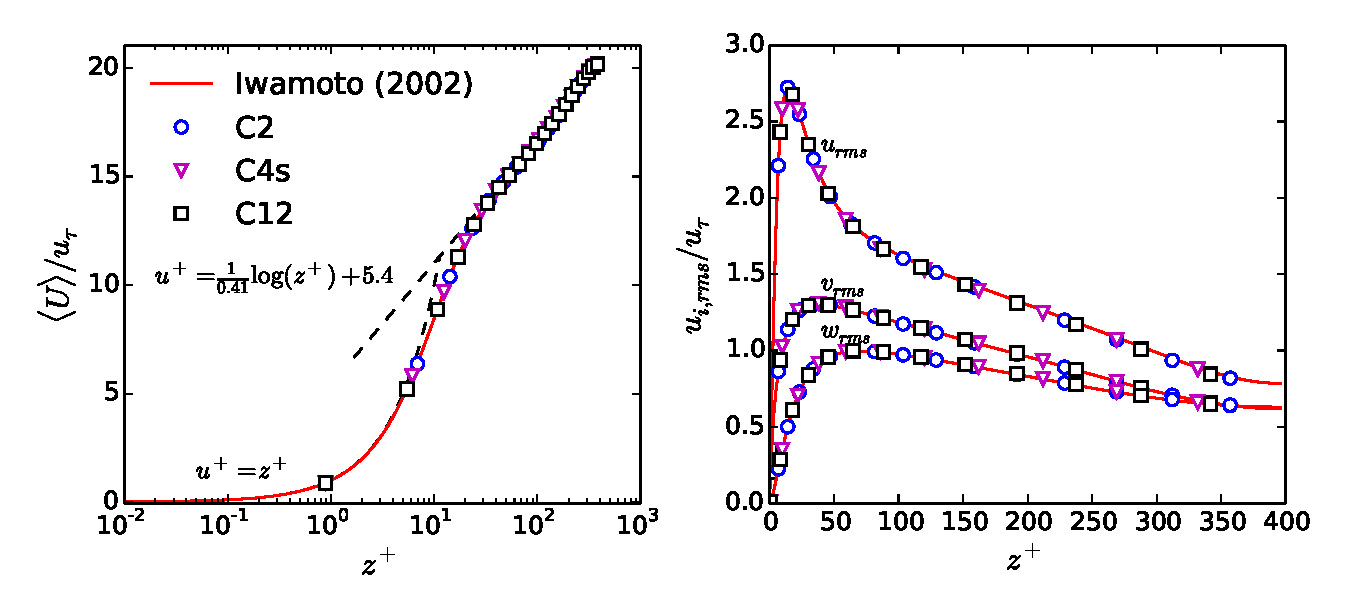
\includegraphics[width=\textwidth,trim= 0cm 0.35cm 0cm 0.3cm,clip]{chapters/pof_shifting/figure3}
	\caption{Comparison of C2, C4$s$ and C12 cases with reference data from Iwamoto \emph{et al.}\cite{iwamoto2002reynolds} Left: Mean streamwise velocity profile. Right: Mean root-mean-square velocity fluctuations. The amount of symbols has been altered for every case solely for clarity.}
	\label{fig:validation}
\end{figure}

Figure~\ref{fig:topviewCHANNEL} shows the plan views of partially time-averaged streamwise velocity fields at a distance $z/\delta = 0.05$ ($z^+ \approx 20$) from the lower wall for each of the channel-flow cases. Averaging times range from $Tu_*/\delta=10$ to $100$, and results are shown for $0\leq x \leq \pi\delta$. The figure illustrates that for the smaller domain cases, i.e. C2 and C4, the locking effect leads to significant banded variations in mean velocity profiles in the spanwise direction. For shorter averaging horizons (i.e. up until $T u_* / \delta = 20$), the partial averages of the longer cases, i.e. C6 and C12, appear very similar to those of the shorter ones. However, for time-averaging windows $Tu_*/\delta \ge 60$, the spanwise inhomogeneity disappears for the longer domains C6 and C12. Note that the longest time-averaging horizon shown in these plots ($Tu_*/\delta=100$) corresponds to approximately 280 flow-through times of the C2 domain. Finally, Figure~\ref{fig:topviewCHANNEL} demonstrates that the shifted cases (C2$s$ and C4$s$) exhibit the same behavior as the C6 and C12 cases, even though the streamwise domain length is significantly smaller. 

\begin{figure}[t]
	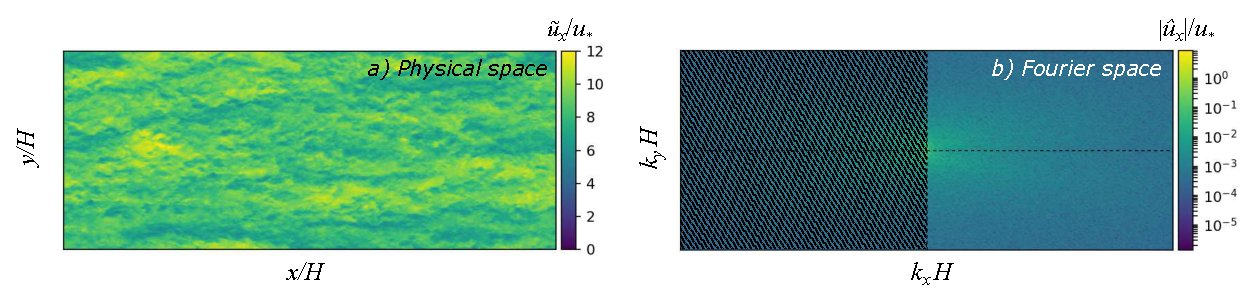
\includegraphics[width=\textwidth]{chapters/pof_shifting/figure4}
	\caption{Planview of time-averaged streamwise velocity in the buffer layer at a height of $z/\delta$ = 0.05 ($z^+ \approx 20$) from the lower wall for the C cases described in Table \ref{tab:cases}. The illustrated domains are truncated in the streamwise direction at $x = \pi\delta$. Coloring is in units of $u/u_*$.}
	\label{fig:topviewCHANNEL}
\end{figure}

Figure \ref{fig:delta_factorCHANNEL} provides a more quantitative illustration of the spanwise inhomogeneities in the simulation with the normalized peak-to-trough variation $\Delta$, defined as
\begin{equation}
	\Delta(x,z,T) = \frac{1}{\langle U \rangle (z,T)} \bigg [ \max_y \{ U(x,y,z,T) \} - \min_y \{ U(x,y,z,T)  \}  \bigg ],
\end{equation}
where U is the time-averaged streamwise velocity over a time window T, and $\langle \cdot \rangle$ denotes a horizontal averaging operation. Note that $\Delta(x,z,T)$ is virtually independent of the streamwise location $x$, hence we will implicitly refer to $\Delta(z,T)$ as the value at the inflow plane, unless stated otherwise. Figure \ref{fig:delta_factorCHANNEL}a shows $\Delta$ at $z/\delta = 0.05$, corresponding to the plan views in Figure \ref{fig:topviewCHANNEL}. It confirms the statement from previous paragraph that, for shorter time windows up to $Tu_*/\delta = 20$, all non-shifted cases seem to have a similar $\Delta$. Longer time averaging decreases $\Delta$, up to a certain point around $Tu_*/\delta = 70$, after which asymptotic behavior is observed. Moreover, the shifted C4$s$ case closely resembles the behavior of the longer periodic C6 and C12 cases. The C2$s$ case finally also reaches the same asymptote as C4$s$, C6 and C12 for large $Tu_*/\delta$. Figure \ref{fig:delta_factorCHANNEL}b illustrates the height-dependence of $\Delta$ for all cases for the longest time-horizon $Tu_*/\delta = 100$. As expected, spanwise variations are highest closer to the channel walls, where velocity fluctuations are strongest. This was also observed by Fishpool et al.\cite{fishpool2009persistent}

\begin{figure}[t]
	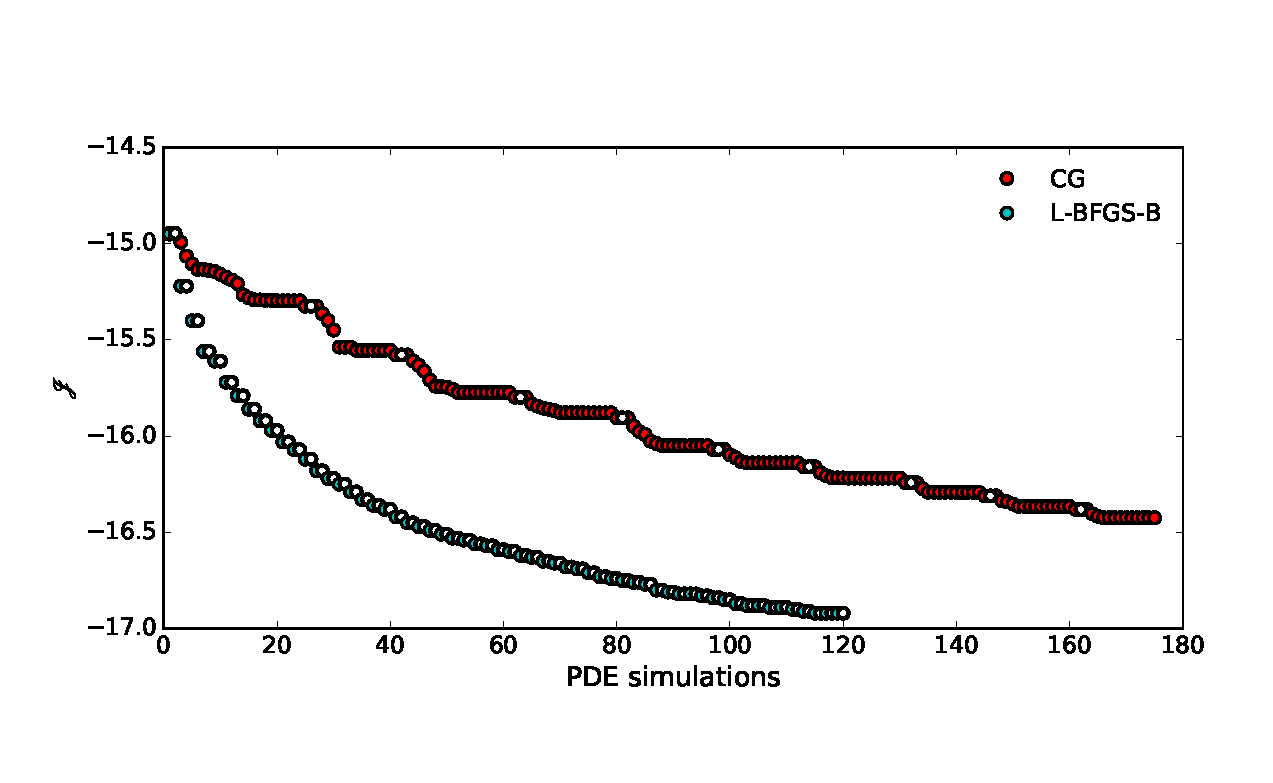
\includegraphics[width=\textwidth, trim= 0cm 0.15cm 0cm 0.cm,clip]{chapters/pof_shifting/figure5}
	\caption{Peak-to-trough spanwise inhomogeneity factor $\Delta$ for the channel flow DNS C cases: \emph{a)} $\Delta$ in function of time-averaging window $Tu_*/\delta$ (at height $z/\delta = 0.05$). \emph{b)} $\Delta$ in function of height $z/\delta$ (at final time-averaging window $Tu_*/\delta = 100$). The dashed line indicates $z/\delta = 0.05$. To increase statistical convergence of \emph{b)}, we averaged over both the streamwise direction and the 2 halves of the channel. }
	\label{fig:delta_factorCHANNEL}
\end{figure}

To conclude the discussion, Figure \ref{fig:correlationsC} shows longitudinal autocorrelations of streamwise velocity $\rho_{uu}$. Since the non-shifted cases (i.e. C2, C4, C6 and C12) apply classical periodic boundary conditions, the autocorrelation of these simulations attain values of 1 at $r_x = L_x$ by definition. This is not the case for the shifted simulations C2$s$ and C4$s$. The C2 case autocorrelation does not reach a zero value over its streamwise domain length, illustrating that the simulation domain is too short. Similarly, the autocorrelation of C4 barely reaches a zero value at $r_x/\delta \approx 2 \pi$, before increasing to unity again. Both these observations show that the domains of C2 and C4 are too short to achieve full decorrelation over the streamwise domain length, explaining the banded structure in Figure \ref{fig:topviewCHANNEL}, and the high $\Delta$-values in Figure \ref{fig:delta_factorCHANNEL}. The longer cases C6 and C12 have an extended region of zero correlations. Both shifted cases, C2$s$ and C4$s$, also achieve decorrelation over their domain length. Moreover, note that C2$s$ and C4$s$ match virtually perfectly with the longer cases over their domain length, indicating that the shifting operation does not have any adverse effects on the longitudinal autocorrelation behavior.

\begin{figure}[t]
	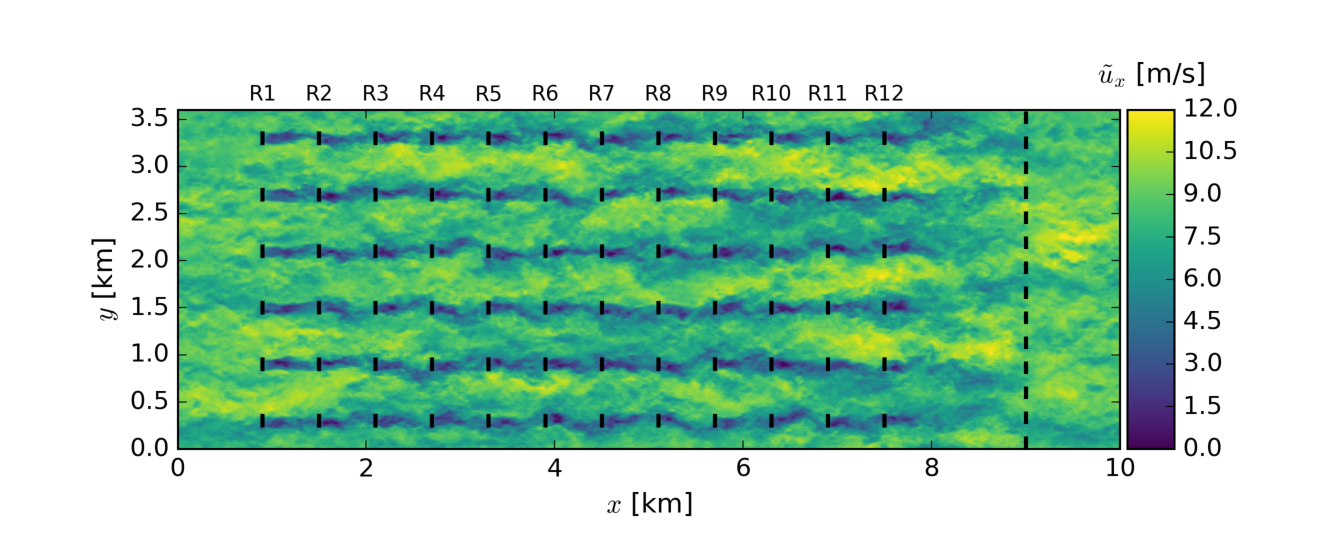
\includegraphics[width=\textwidth,trim= 0cm 0.2cm 0cm 0.cm,clip]{chapters/pof_shifting/figure6}
	\caption{One-dimensional longitudinal autocorrelations $\rho_{uu}(r_x)$ at $z/\delta = 0.05$ for the C cases. The vertical black dotted lines represent the domain lengths of the shorter cases, i.e. $L_x = 2\pi\delta$, $4\pi\delta$ and $6\pi\delta$, from left to right.}
	\label{fig:correlationsC}
\end{figure}

\subsection{Fully-developed high-Reynolds number half-channel flow}

We now turn to the simulation results of the high Reynolds-number half-channel (HC) cases. Figure~\ref{fig:topviewHC} shows plan views of partially time-averaged streamwise velocity fields at a distance $z/\delta = 0.1$ from the surface. Firstly, note that the color range for the HC cases in this figure is significantly wider than for the C cases shown in Figure \ref{fig:topviewCHANNEL}. For this much higher Reynolds number, it is observed that even the longest HC12 case is influenced by the spanwise locking of structures, though it should be noted that the effect is much smaller than for the HC1 and HC2 cases. This is not unexpected, as VLSM in high-Reynolds number boundary layers carry more kinetic energy and tend to be longer than those observed at low Reynolds numbers,\cite{balakumar2007large,hutchins2007evidence,hutchins2007large,hutchins2012towards} e.g., structures of size $20\delta$ have been reported in LES of the atmospheric boundary layer.\cite{fang2015large} 
Looking at the results from the shifted periodic boundary condition cases HC2$s$ and HC4$s$ in Figure~\ref{fig:topviewHC}, it is seen that the spanwise inhomogeneities are reduced from the outset onwards, leading to results that are even more homogeneous than the HC12 case, even though domain lengths are significantly shorter. 

% Topview of channel flows
\begin{figure}[t]
	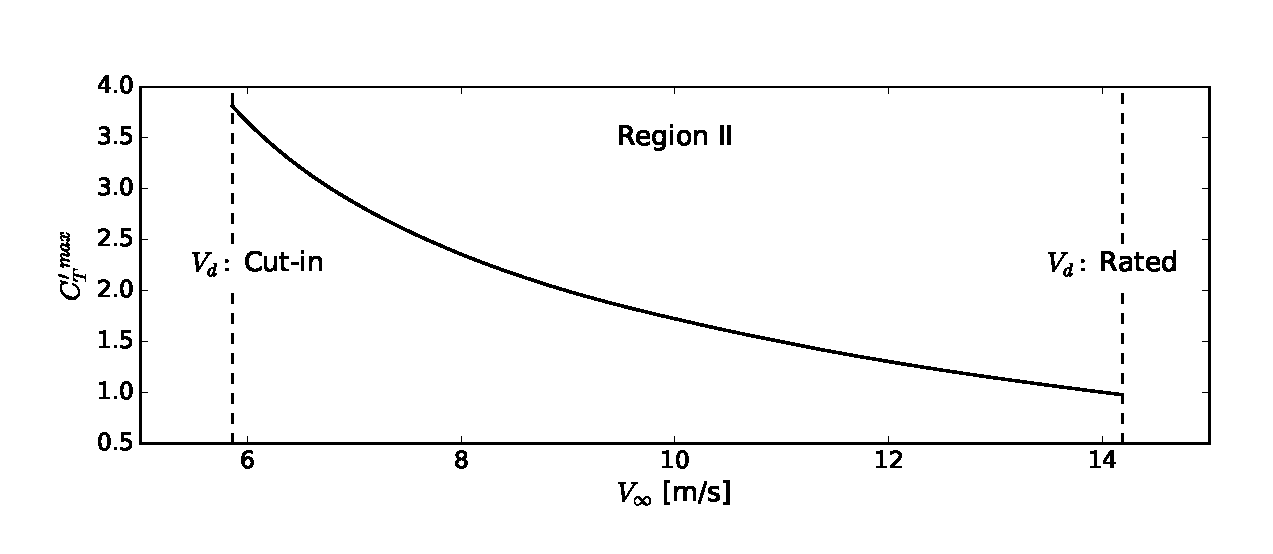
\includegraphics[width=\textwidth]{chapters/pof_shifting/figure7}
	\caption{Planview of time-averaged streamwise velocity in the log-law region at a height of $z/\delta$ = 0.1 ($z/z_0 = 10^3$) from the surface for the HC cases described in Table \ref{tab:cases}. The illustrated domains are truncated in the streamwise direction at $x = \pi$. Coloring is in units of  $u/u_*$.}
	\label{fig:topviewHC}
\end{figure}

Figure \ref{fig:delta_factorHC} illustrates the $\Delta$-factor described above for the HC cases. Figure \ref{fig:delta_factorHC}a again shows the dependency of $\Delta$ on the time-averaging window $Tu_*/\delta$ at a height $z/\delta = 0.1$, corresponding to the plan views in Figure \ref{fig:topviewHC}. It can be seen that the shifted cases HC2$s$ and HC4$s$ show consistently lower inhomogeneities which, at the longest time-window $Tu_*/\delta = 60$, are approximately an order of magnitude lower than the non-shifted cases, the latter equalling roughly 10\% of the time-averaged mean velocity at the same height. Figure \ref{fig:delta_factorHC}b illustrates the height dependence of $\Delta$ at the longest time-window. Generally, the highest $\Delta$-values can again be found closer to the wall (except for the very short HC1 case), although the reduction of $\Delta$ away from the wall is much lower than in the low Reynolds number case. 

\begin{figure}[t]
	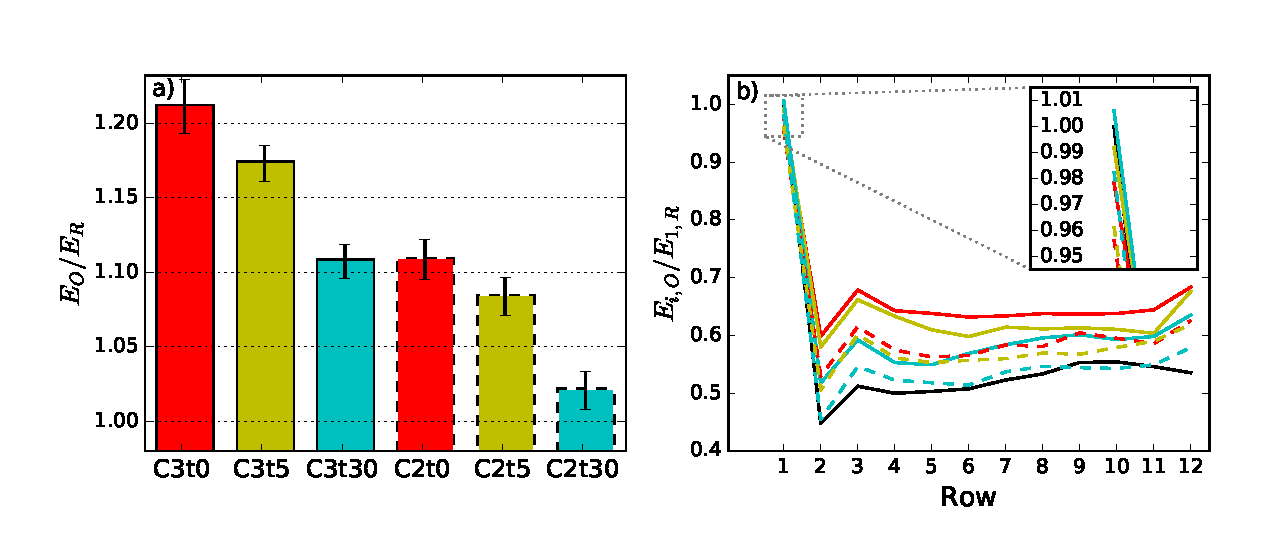
\includegraphics[width=\textwidth, trim= 0cm 0.15cm 0cm 0.cm,clip]{chapters/pof_shifting/figure8}
	\caption{Peak-to-trough spanwise inhomogeneity factor $\Delta$ for the half-channel flow LES HC cases: \emph{a)} $\Delta$ in function of time-averaging window $Tu_*/\delta$ (at height $z/\delta = 0.1$). \emph{b)} $\Delta$ in function of height $z/\delta$ (at final time-averaging window $Tu_*/\delta = 60$). The dashed line indicates $z/\delta = 0.1$.}
	\label{fig:delta_factorHC}
\end{figure}
	
Figure \ref{fig:correlations} illustrates longitudinal autocorrelations $\rho_{uu}$ for each of the HC cases. Similar to the C cases from previous section, the non-shifted cases  are perfectly correlated at $r_x = L_x$ due to the periodic boundary conditions. Moreover, except for HC12, all conventionally periodic cases fail to achieve decorrelation of turbulent structures over their streamwise domain length (e.g. for the HC2 case with a conventional domain length $L_x = 2\pi\delta$,  $\rho_{uu}$ does not drop below 0.2), which suggests the presence and persistence of domain-scale coherent structures. Although HC12 reaches $\rho_{uu} = 0$ at $r_x/\delta = 6\pi$, this is not sufficient to avoid the locking effect, as was also observed in case C4 of the previous section. The shifted cases HC2$s$ and HC4$s$ however  clearly show decorrelation between the inlet and outlet of the domain. The negative values of $\rho_{uu}$ at $r_x = L_x$ can be attributed to a combination of a spanwise shift length $d_s = 0.5 \delta$ and the negatively correlated counter-rotating vortices neighboring the VLSM in the spanwise direction (see, e.g. Refs \cite{tomkins2003spanwise, hutchins2012towards} , transversal correlations omitted here for brevity). Finally, note that the HC4$s$ case achieves a zero-crossing of $\rho_{uu}$ at $r_x/\delta \approx 10$.  This is consistent with the recently obtained results of Fang \& Port\'e-Agel,\cite{fang2015large} who performed a very similar case on a much larger domain ($L_x = 32\pi\delta$, $L_y = 4\pi\delta$). This suggests that a simulation domain with streamwise length $L_x = 4\pi\delta$, combined with shifted periodic boundary conditions, produces coherent turbulent structures with the same autocorrelation behavior as the ones observed in much larger domains. 

\begin{figure}[t]
	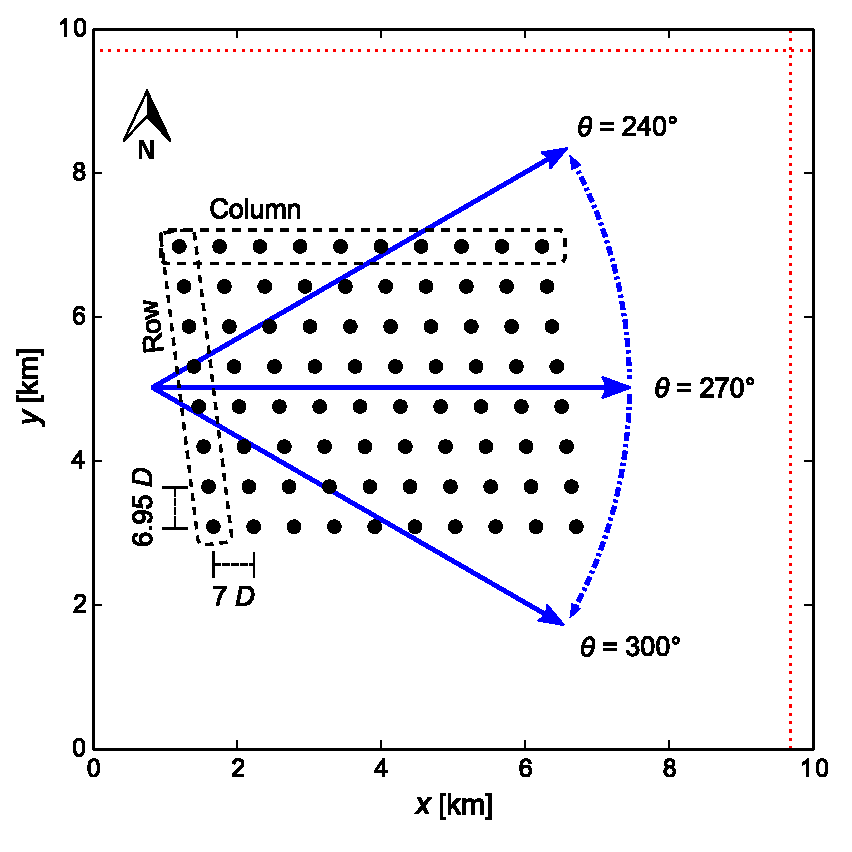
\includegraphics[width=\textwidth,trim= 0cm 0.2cm 0cm 0.cm,clip]{chapters/pof_shifting/figure9}
	\caption{One-dimensional longitudinal autocorrelations $\rho_{uu}(r_x)$ at $z/\delta = 0.1$ for the HC cases. The vertical black dotted lines represent the domain lengths of the shorter cases, i.e. $L_x = \pi$, $2\pi$, $4\pi$ and $6\pi$, from left to right.}
	\label{fig:correlations}
\end{figure}

Finally, we present the method's dependency on the user-defined shifting distance $d_s$ in Figure \ref{fig:ds_dependency}. Here, we show the spanwise profiles of time-averaged streamwise velocity component for the cases HC2$s$ and HC2 defined above, as well as four additional shifted cases simulated on the HC2$s$ domain with a range of $d_s$ values. Profiles are illustrated at a height $z/\delta = 0.1$ for a time-averaging window $Tu_*/\delta = 20$. The figure illustrates that satisfactory results are also obtained for $d_s = \delta/4$, $\delta$, and $d_s = 3\delta/2$. For completeness, we include a case with $d_s = L_y/2$ as an example of a poor choice of shifting distance (see discussion in Section \ref{sec:methodology}). It is observed that, for the latter case, inhomogeneities are replicated to multiple spanwise locations while they are only marginally attenuated.

\begin{figure}[t]
	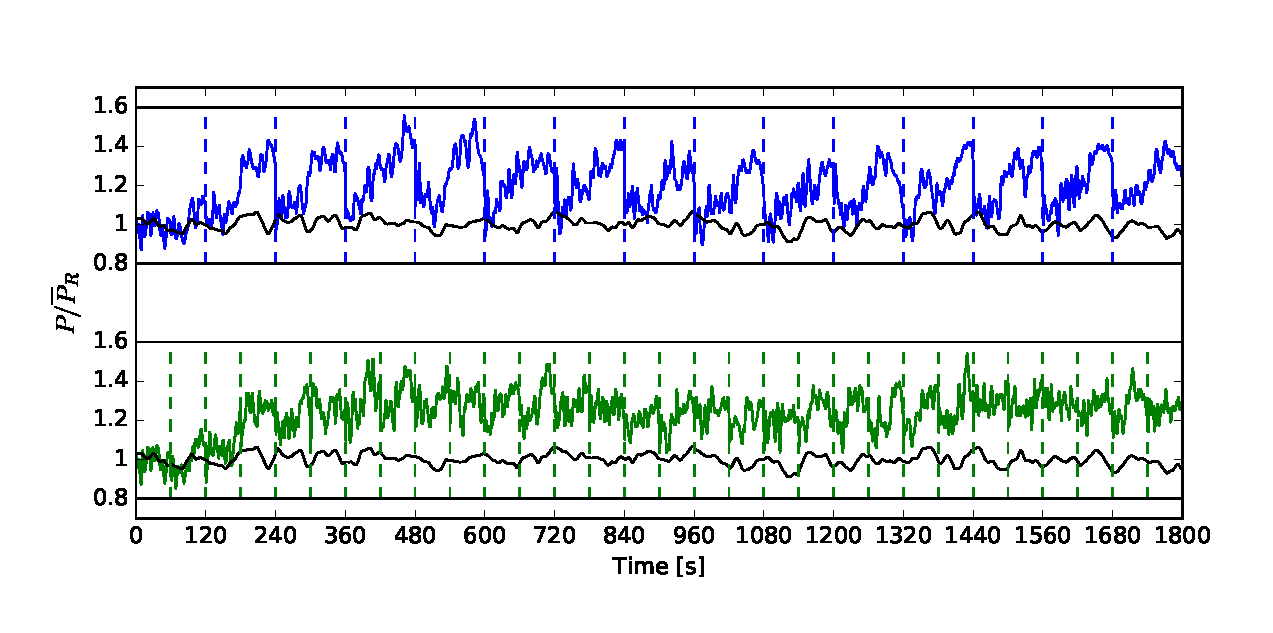
\includegraphics[width=\textwidth,, trim = 0 10 0 10,clip]{chapters/pof_shifting/figure10}
	\caption{Time-averaged streamwise velocity component at $z/\delta = 0.1$ as a function of spanwise location for various shifting distances $d_s$. Profiles are averaged over the streamwise direction and normalized by their horizontally-averaged values. Time averages calculated for a window of $Tu_*/\delta = 20$.}
	\label{fig:ds_dependency}
\end{figure}


% % % % % % % % % % % % % % % % % % % % % % % % % % % % % % % % % % % % % % % % % % 
\section{Application to large-eddy simulation of a spatially developing wind-farm boundary layer}\label{sec:windfarm}
% % % % % % % % % % % % % % % % % % % % % % % % % % % % % % % % % % % % % % % % % % 

As shown in previous paragraph, shifted periodic boundary conditions can effectively reduce spanwise variations of physically spanwise-homogeneous flows that are simulated on relatively short domains. We conclude this manuscript with an application case of atmospheric boundary layer flow through a wind farm. The HC2, HC4, HC4$s$, HC6, and HC12 cases defined above are used as precursor simulations, providing inflow conditions to a main simulation domain with dimensions $L_x \times L_y \times H = 1.5\pi \delta \times 2\pi \delta \times \delta$. Actuator disk models\cite{mikkelsen2003actuator} are used to represent a $4 \times 12$ array of wind turbines with hub height $z_h/\delta = 0.10$, turbine diameter $D/\delta = 0.10$ and turbine thrust coefficient\cite{calaf2010large} $C_T' = 4/3$ (see Figure \ref{fig:WF}a). The grid resolution and turbine spacing ($S_x = 7.85D$, $S_x/S_y = 1.5$) correspond to the well-established A1 base case from Calaf \emph{et al.}\cite{calaf2010large} In the following discussion, a column (row) is defined as a set of turbines located at the same spanwise (streamwise) coordinate.
Simulation results are shown in Figure~\ref{fig:WF}. The simulations were performed for a time horizon of $Tu_*/\delta = 15$, corresponding to a physical time of slightly over 8 hours for typical atmospheric conditions ($u_* = 0.5$ m s$^{-1}$, $\delta = 1000$ m). Figure~\ref{fig:WF}a shows time-averaged contours of streamwise velocity at hub height, using the HC2 case as inflow generator. As shown in the figure, the spanwise locking effect of streamwise-elongated structures leads to an unrealistic distribution of high and low velocity regions among the different turbine columns in the wind farm, which in turn causes the large differences in power extraction between columns, as shown in Figure~\ref{fig:WF}b. As further observed in Figures \ref{fig:WF}c and \ref{fig:WF}d, when employing a shifted periodic boundary condition in the precursor domain (i.e. HC4$s$) this spanwise inhomogeneity in averages disappears over long time averages. 

\begin{figure}
	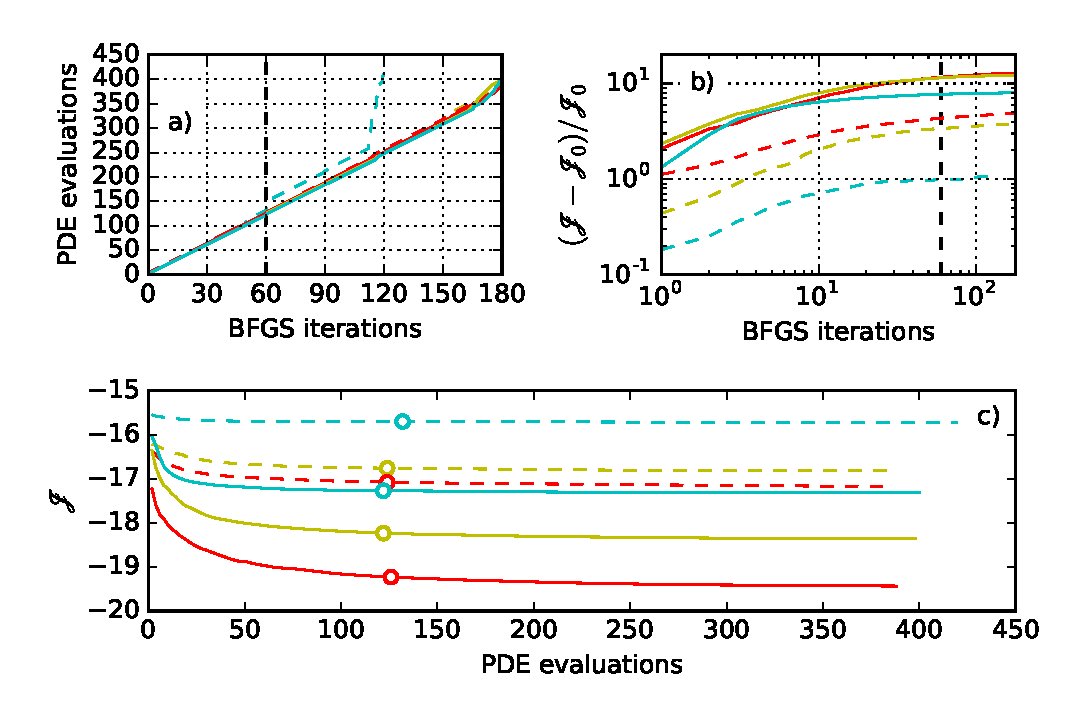
\includegraphics[width=\textwidth]{chapters/pof_shifting/figure11}
	\caption{Wind-farm demo cases. \emph{a)} \& \emph{c)}: Planview of time-averaged flow field using HC2 (\emph{a}) and HC4$s$ (\emph{c}) as inflow simulation. \emph{b)} \& \emph{d)}: Time-averaged turbine power for different columns for non-shifted cases (\emph{b}), and shifted HC4$s$ case (\emph{d}). Powers are normalized by farm-averaged power (dashed black lines). Cases are shifted vertically for clarity. Dotted black lines indicate deviations of $\pm$10\% from the farm average.}
	\label{fig:WF}
\end{figure}

\section{Conclusion}\label{sec:conclusion}
This manuscript describes a simple yet efficient method to avoid the persistent spanwise locking of large-scale turbulent flow structures in canonical wall-bounded flow simulations with periodic lateral boundary conditions. The shifted periodic boundary condition approach replaces the streamwise periodicity by a spanwise shifted one, hence distributing turbulent structures amongst spanwise locations. The method is effective in obtaining better spanwise convergence of time-averaged flow fields for various flow cases and simulation strategies, as illustrated by a suite of low Reynolds number channel flows using direct numerical simulation and very high Reynolds number half-channel flows using large-eddy simulation. A wind-farm demonstration case showed one of many possible practical applications in which the method is useful.

Finally, we remark that the use of a fully-developed precursor simulation with classical periodic boundary conditions as an inflow generator for cases with significant streamwise development can yield undesirable effects. More specifically, Lund, Wu and Squires\cite{lund1998generation} report underpredicted growth rates and spurious inlet development regions for the case of a developing flat-plate turbulent boundary layer. Similar effects were observed by Lund and Moin\cite{lund1996large} for the case of a concave wall boundary layer. They hypothesized that these phenomena could be related to an artificially high degree of streamwise coherence in the inflow data, resulting from the application of periodic boundary conditions to a relatively short precursor domain. Therefore, an interesting topic for future research could be to assess whether a shifted periodic boundary condition could overcome this ailment of its traditional counterpart. 



% % % % % % % % % % % % % % % % % % % % % % % % % % % % % % % % % % % % % % % % % % % % % % % % % % % % % % % %
\section*{Acknowledgements}
We thank Dr. R. Stevens and Dr. A. \"Onder for useful discussions. WM and JM are supported by the ERC (ActiveWindFarms, grant no: 306471). CM acknowledges support by the NSF (grant IIA-1243482, the WINDINSPIRE project).
The computational resources and services used in this work were provided by the VSC (Flemish Supercomputer Center), funded by the Hercules Foundation and the Flemish Government - department EWI.

%\bibliography{mybibfile_abbrev}
%merlin.mbs aipnum4-1.bst 2010-07-25 4.21a (PWD, AO, DPC) hacked
%Control: key (0)
%Control: author (8) initials jnrlst
%Control: editor formatted (1) identically to author
%Control: production of article title (0) allowed
%Control: page (1) range
%Control: year (1) truncated
%Control: production of eprint (0) enabled
\begin{thebibliography}{36}%
\makeatletter
\providecommand \@ifxundefined [1]{%
 \@ifx{#1\undefined}
}%
\providecommand \@ifnum [1]{%
 \ifnum #1\expandafter \@firstoftwo
 \else \expandafter \@secondoftwo
 \fi
}%
\providecommand \@ifx [1]{%
 \ifx #1\expandafter \@firstoftwo
 \else \expandafter \@secondoftwo
 \fi
}%
\providecommand \natexlab [1]{#1}%
\providecommand \enquote  [1]{``#1''}%
\providecommand \bibnamefont  [1]{#1}%
\providecommand \bibfnamefont [1]{#1}%
\providecommand \citenamefont [1]{#1}%
\providecommand \href@noop [0]{\@secondoftwo}%
\providecommand \href [0]{\begingroup \@sanitize@url \@href}%
\providecommand \@href[1]{\@@startlink{#1}\@@href}%
\providecommand \@@href[1]{\endgroup#1\@@endlink}%
\providecommand \@sanitize@url [0]{\catcode `\\12\catcode `\$12\catcode
  `\&12\catcode `\#12\catcode `\^12\catcode `\_12\catcode `\%12\relax}%
\providecommand \@@startlink[1]{}%
\providecommand \@@endlink[0]{}%
\providecommand \url  [0]{\begingroup\@sanitize@url \@url }%
\providecommand \@url [1]{\endgroup\@href {#1}{\urlprefix }}%
\providecommand \urlprefix  [0]{URL }%
\providecommand \Eprint [0]{\href }%
\providecommand \doibase [0]{http://dx.doi.org/}%
\providecommand \selectlanguage [0]{\@gobble}%
\providecommand \bibinfo  [0]{\@secondoftwo}%
\providecommand \bibfield  [0]{\@secondoftwo}%
\providecommand \translation [1]{[#1]}%
\providecommand \BibitemOpen [0]{}%
\providecommand \bibitemStop [0]{}%
\providecommand \bibitemNoStop [0]{.\EOS\space}%
\providecommand \EOS [0]{\spacefactor3000\relax}%
\providecommand \BibitemShut  [1]{\csname bibitem#1\endcsname}%
\let\auto@bib@innerbib\@empty
%</preamble>
\bibitem [{\citenamefont {Kim}, \citenamefont {Moin},\ and\ \citenamefont
  {Moser}(1987)}]{kim1987turbulence}%
  \BibitemOpen
  \bibfield  {author} {\bibinfo {author} {\bibfnamefont {J.}~\bibnamefont
  {Kim}}, \bibinfo {author} {\bibfnamefont {P.}~\bibnamefont {Moin}}, \ and\
  \bibinfo {author} {\bibfnamefont {R.}~\bibnamefont {Moser}},\ }\bibfield
  {title} {\enquote {\bibinfo {title} {Turbulence statistics in fully developed
  channel flow at low Reynolds number},}\ }\href@noop {} {\bibfield  {journal}
  {\bibinfo  {journal} {J Fluid Mech}\ }\textbf {\bibinfo {volume} {177}},\
  \bibinfo {pages} {133--166} (\bibinfo {year} {1987})}\BibitemShut {NoStop}%
\bibitem [{\citenamefont {Monty}\ \emph {et~al.}(2007)\citenamefont {Monty},
  \citenamefont {Stewart}, \citenamefont {Williams},\ and\ \citenamefont
  {Chong}}]{monty2007large}%
  \BibitemOpen
  \bibfield  {author} {\bibinfo {author} {\bibfnamefont {J.}~\bibnamefont
  {Monty}}, \bibinfo {author} {\bibfnamefont {J.}~\bibnamefont {Stewart}},
  \bibinfo {author} {\bibfnamefont {R.}~\bibnamefont {Williams}}, \ and\
  \bibinfo {author} {\bibfnamefont {M.}~\bibnamefont {Chong}},\ }\bibfield
  {title} {\enquote {\bibinfo {title} {Large-scale features in turbulent pipe
  and channel flows},}\ }\href@noop {} {\bibfield  {journal} {\bibinfo
  {journal} {J Fluid Mech}\ }\textbf {\bibinfo {volume} {589}},\ \bibinfo
  {pages} {147--156} (\bibinfo {year} {2007})}\BibitemShut {NoStop}%
\bibitem [{\citenamefont {Wu}\ and\ \citenamefont {Moin}(2008)}]{wu2008direct}%
  \BibitemOpen
  \bibfield  {author} {\bibinfo {author} {\bibfnamefont {X.}~\bibnamefont
  {Wu}}\ and\ \bibinfo {author} {\bibfnamefont {P.}~\bibnamefont {Moin}},\
  }\bibfield  {title} {\enquote {\bibinfo {title} {A direct numerical
  simulation study on the mean velocity characteristics in turbulent pipe
  flow},}\ }\href@noop {} {\bibfield  {journal} {\bibinfo  {journal} {J Fluid
  Mech}\ }\textbf {\bibinfo {volume} {608}},\ \bibinfo {pages} {81--112}
  (\bibinfo {year} {2008})}\BibitemShut {NoStop}%
\bibitem [{\citenamefont {Tsukahara}, \citenamefont {Kawamura},\ and\
  \citenamefont {Shingai}(2006)}]{takahiro2006dns}%
  \BibitemOpen
  \bibfield  {author} {\bibinfo {author} {\bibfnamefont {T.}~\bibnamefont
  {Tsukahara}}, \bibinfo {author} {\bibfnamefont {H.}~\bibnamefont {Kawamura}},
  \ and\ \bibinfo {author} {\bibfnamefont {K.}~\bibnamefont {Shingai}},\
  }\bibfield  {title} {\enquote {\bibinfo {title} {{DNS} of turbulent {C}ouette
  flow with emphasis on the large-scale structure in the core region},}\
  }\href@noop {} {\bibfield  {journal} {\bibinfo  {journal} {J Turbul}\
  }\textbf {\bibinfo {volume} {7}},\ \bibinfo {pages} {N19, 16 pp.} (\bibinfo {year}
  {2006})}\BibitemShut {NoStop}%
\bibitem [{\citenamefont {Tabor}\ and\ \citenamefont
  {Baba-Ahmadi}(2010)}]{tabor2010inlet}%
  \BibitemOpen
  \bibfield  {author} {\bibinfo {author} {\bibfnamefont {G.}~\bibnamefont
  {Tabor}}\ and\ \bibinfo {author} {\bibfnamefont {M.}~\bibnamefont
  {Baba-Ahmadi}},\ }\bibfield  {title} {\enquote {\bibinfo {title} {Inlet
  conditions for large eddy simulation: a review},}\ }\href@noop {} {\bibfield
  {journal} {\bibinfo  {journal} {Comput Fluids}\ }\textbf {\bibinfo {volume}
  {39}},\ \bibinfo {pages} {553--567} (\bibinfo {year} {2010})}\BibitemShut
  {NoStop}%
\bibitem [{\citenamefont {Stevens}, \citenamefont {Graham},\ and\ \citenamefont
  {Meneveau}(2014)}]{stevens2014concurrent}%
  \BibitemOpen
  \bibfield  {author} {\bibinfo {author} {\bibfnamefont {R.~J. A.~M.}\
  \bibnamefont {Stevens}}, \bibinfo {author} {\bibfnamefont {J.}~\bibnamefont
  {Graham}}, \ and\ \bibinfo {author} {\bibfnamefont {C.}~\bibnamefont
  {Meneveau}},\ }\bibfield  {title} {\enquote {\bibinfo {title} {A concurrent
  precursor inflow method for large eddy simulations and applications to finite
  length wind farms},}\ }\href@noop {} {\bibfield  {journal} {\bibinfo
  {journal} {Renew Energ}\ }\textbf {\bibinfo {volume} {68}},\ \bibinfo {pages}
  {46--50} (\bibinfo {year} {2014})}\BibitemShut {NoStop}%
\bibitem [{\citenamefont {Del~{\'A}lamo}\ and\ \citenamefont
  {Jim{\'e}nez}(2003)}]{delalamo2003spectra}%
  \BibitemOpen
  \bibfield  {author} {\bibinfo {author} {\bibfnamefont {J.~C.}\ \bibnamefont
  {Del~{\'A}lamo}}\ and\ \bibinfo {author} {\bibfnamefont {J.}~\bibnamefont
  {Jim{\'e}nez}},\ }\bibfield  {title} {\enquote {\bibinfo {title} {Spectra of
  the very large anisotropic scales in turbulent channels},}\ }\href@noop {}
  {\bibfield  {journal} {\bibinfo  {journal} {Phys Fluids}\ }\textbf {\bibinfo
  {volume} {15}},\ \bibinfo {pages} {L41} (\bibinfo {year} {2003})}\BibitemShut
  {NoStop}%
\bibitem [{\citenamefont {Del~{\'A}lamo}\ \emph {et~al.}(2004)\citenamefont
  {Del~{\'A}lamo}, \citenamefont {Jim{\'e}nez}, \citenamefont {Zandonade},\
  and\ \citenamefont {Moser}}]{delalamo2004scaling}%
  \BibitemOpen
  \bibfield  {author} {\bibinfo {author} {\bibfnamefont {J.~C.}\ \bibnamefont
  {Del~{\'A}lamo}}, \bibinfo {author} {\bibfnamefont {J.}~\bibnamefont
  {Jim{\'e}nez}}, \bibinfo {author} {\bibfnamefont {P.}~\bibnamefont
  {Zandonade}}, \ and\ \bibinfo {author} {\bibfnamefont {R.~D.}\ \bibnamefont
  {Moser}},\ }\bibfield  {title} {\enquote {\bibinfo {title} {Scaling of the
  energy spectra of turbulent channels},}\ }\href@noop {} {\bibfield  {journal}
  {\bibinfo  {journal} {J Fluid Mech}\ }\textbf {\bibinfo {volume} {500}},\
  \bibinfo {pages} {135--144} (\bibinfo {year} {2004})}\BibitemShut {NoStop}%
\bibitem [{\citenamefont {Jim{\'e}nez}(1998)}]{jimenez1998largest}%
  \BibitemOpen
  \bibfield  {author} {\bibinfo {author} {\bibfnamefont {J.}~\bibnamefont
  {Jim{\'e}nez}},\ }\bibfield  {title} {\enquote {\bibinfo {title} {The largest
  scales of turbulent wall flows},}\ }\href@noop {} {\bibfield  {journal}
  {\bibinfo  {journal} {CTR Annual Research Briefs}\ }\textbf {\bibinfo
  {volume} {137}},\ \bibinfo {pages} {54} (\bibinfo {year} {1998})}\BibitemShut
  {NoStop}%
\bibitem [{\citenamefont {Tomkins}\ and\ \citenamefont
  {Adrian}(2003)}]{tomkins2003spanwise}%
  \BibitemOpen
  \bibfield  {author} {\bibinfo {author} {\bibfnamefont {C.~D.}\ \bibnamefont
  {Tomkins}}\ and\ \bibinfo {author} {\bibfnamefont {R.~J.}\ \bibnamefont
  {Adrian}},\ }\bibfield  {title} {\enquote {\bibinfo {title} {Spanwise
  structure and scale growth in turbulent boundary layers},}\ }\href@noop {}
  {\bibfield  {journal} {\bibinfo  {journal} {J Fluid Mech}\ }\textbf {\bibinfo
  {volume} {490}},\ \bibinfo {pages} {37--74} (\bibinfo {year}
  {2003})}\BibitemShut {NoStop}%
\bibitem [{\citenamefont {Hutchins}\ and\ \citenamefont
  {Marusic}(2007{\natexlab{a}})}]{hutchins2007evidence}%
  \BibitemOpen
  \bibfield  {author} {\bibinfo {author} {\bibfnamefont {N.}~\bibnamefont
  {Hutchins}}\ and\ \bibinfo {author} {\bibfnamefont {I.}~\bibnamefont
  {Marusic}},\ }\bibfield  {title} {\enquote {\bibinfo {title} {Evidence of
  very long meandering features in the logarithmic region of turbulent boundary
  layers},}\ }\href@noop {} {\bibfield  {journal} {\bibinfo  {journal} {J Fluid
  Mech}\ }\textbf {\bibinfo {volume} {579}},\ \bibinfo {pages} {1--28}
  (\bibinfo {year} {2007}{\natexlab{a}})}\BibitemShut {NoStop}%
\bibitem [{\citenamefont {Lu}\ and\ \citenamefont
  {Port{\'e}-Agel}(2010)}]{lu2010modulated}%
  \BibitemOpen
  \bibfield  {author} {\bibinfo {author} {\bibfnamefont {H.}~\bibnamefont
  {Lu}}\ and\ \bibinfo {author} {\bibfnamefont {F.}~\bibnamefont
  {Port{\'e}-Agel}},\ }\bibfield  {title} {\enquote {\bibinfo {title} {A
  modulated gradient model for large-eddy simulation: Application to a neutral
  atmospheric boundary layer},}\ }\href@noop {} {\bibfield  {journal} {\bibinfo
   {journal} {Phys Fluids}\ }\textbf {\bibinfo {volume} {22}},\
  \bibinfo {eid} {015109} (\bibinfo {year} {2010})}\BibitemShut {NoStop}%
\bibitem [{\citenamefont {Lozano-Dur{\'a}n}\ and\ \citenamefont
  {Jim{\'e}nez}(2014)}]{lozanoduran2014effect}%
  \BibitemOpen
  \bibfield  {author} {\bibinfo {author} {\bibfnamefont {A.}~\bibnamefont
  {Lozano-Dur{\'a}n}}\ and\ \bibinfo {author} {\bibfnamefont {J.}~\bibnamefont
  {Jim{\'e}nez}},\ }\bibfield  {title} {\enquote {\bibinfo {title} {Effect of
  the computational domain on direct simulations of turbulent channels up to
  {${Re}_\tau$} = 4200},}\ }\href@noop {} {\bibfield  {journal} {\bibinfo
  {journal} {Phys Fluids}\ }\textbf {\bibinfo {volume} {26}},\
  \bibinfo {eid} {011702} (\bibinfo {year} {2014})}\BibitemShut {NoStop}%
\bibitem [{\citenamefont {Balakumar}\ and\ \citenamefont
  {Adrian}(2007)}]{balakumar2007large}%
  \BibitemOpen
  \bibfield  {author} {\bibinfo {author} {\bibfnamefont {B.}~\bibnamefont
  {Balakumar}}\ and\ \bibinfo {author} {\bibfnamefont {R.}~\bibnamefont
  {Adrian}},\ }\bibfield  {title} {\enquote {\bibinfo {title} {Large-and
  very-large-scale motions in channel and boundary-layer flows},}\ }\href@noop
  {} {\bibfield  {journal} {\bibinfo  {journal} {Philos T Roy Soc A}\ }\textbf
  {\bibinfo {volume} {365}},\ \bibinfo {pages} {665--681} (\bibinfo {year}
  {2007})}\BibitemShut {NoStop}%
\bibitem [{\citenamefont {Hutchins}\ \emph {et~al.}(2012)\citenamefont
  {Hutchins}, \citenamefont {Chauhan}, \citenamefont {Marusic}, \citenamefont
  {Monty},\ and\ \citenamefont {Klewicki}}]{hutchins2012towards}%
  \BibitemOpen
  \bibfield  {author} {\bibinfo {author} {\bibfnamefont {N.}~\bibnamefont
  {Hutchins}}, \bibinfo {author} {\bibfnamefont {K.}~\bibnamefont {Chauhan}},
  \bibinfo {author} {\bibfnamefont {I.}~\bibnamefont {Marusic}}, \bibinfo
  {author} {\bibfnamefont {J.}~\bibnamefont {Monty}}, \ and\ \bibinfo {author}
  {\bibfnamefont {J.}~\bibnamefont {Klewicki}},\ }\bibfield  {title} {\enquote
  {\bibinfo {title} {Towards reconciling the large-scale structure of turbulent
  boundary layers in the atmosphere and laboratory},}\ }\href@noop {}
  {\bibfield  {journal} {\bibinfo  {journal} {Boundary-Layer Meteorol}\
  }\textbf {\bibinfo {volume} {145}},\ \bibinfo {pages} {273--306} (\bibinfo
  {year} {2012})}\BibitemShut {NoStop}%
\bibitem [{\citenamefont {Kim}\ and\ \citenamefont
  {Adrian}(1999)}]{kim1999very}%
  \BibitemOpen
  \bibfield  {author} {\bibinfo {author} {\bibfnamefont {K.}~\bibnamefont
  {Kim}}\ and\ \bibinfo {author} {\bibfnamefont {R.}~\bibnamefont {Adrian}},\
  }\bibfield  {title} {\enquote {\bibinfo {title} {Very large-scale motion in
  the outer layer},}\ }\href@noop {} {\bibfield  {journal} {\bibinfo  {journal}
  {Phys Fluids}\ }\textbf {\bibinfo {volume} {11}},\ \bibinfo
  {pages} {417--422} (\bibinfo {year} {1999})}\BibitemShut {NoStop}%
\bibitem [{\citenamefont {Fang}\ and\ \citenamefont
  {Port{\'e}-Agel}(2015)}]{fang2015large}%
  \BibitemOpen
  \bibfield  {author} {\bibinfo {author} {\bibfnamefont {J.}~\bibnamefont
  {Fang}}\ and\ \bibinfo {author} {\bibfnamefont {F.}~\bibnamefont
  {Port{\'e}-Agel}},\ }\bibfield  {title} {\enquote {\bibinfo {title}
  {Large-eddy simulation of very-large-scale motions in the neutrally
  stratified atmospheric boundary layer},}\ }\href@noop {} {\bibfield
  {journal} {\bibinfo  {journal} {Boundary-Layer Meteorol}\ }\textbf {\bibinfo
  {volume} {155}},\ \bibinfo {pages} {397--416} (\bibinfo {year}
  {2015})}\BibitemShut {NoStop}%
\bibitem [{\citenamefont {Finnigan}, \citenamefont {Shaw},\ and\ \citenamefont
  {Patton}(2009)}]{finnigan2009turbulence}%
  \BibitemOpen
  \bibfield  {author} {\bibinfo {author} {\bibfnamefont {J.~J.}\ \bibnamefont
  {Finnigan}}, \bibinfo {author} {\bibfnamefont {R.~H.}\ \bibnamefont {Shaw}},
  \ and\ \bibinfo {author} {\bibfnamefont {E.~G.}\ \bibnamefont {Patton}},\
  }\bibfield  {title} {\enquote {\bibinfo {title} {Turbulence structure above a
  vegetation canopy},}\ }\href@noop {} {\bibfield  {journal} {\bibinfo
  {journal} {J Fluid Mech}\ }\textbf {\bibinfo {volume} {637}},\ \bibinfo
  {pages} {387--424} (\bibinfo {year} {2009})}\BibitemShut {NoStop}%
\bibitem [{\citenamefont {VerHulst}\ and\ \citenamefont
  {Meneveau}(2014)}]{verhulst2014large}%
  \BibitemOpen
  \bibfield  {author} {\bibinfo {author} {\bibfnamefont {C.}~\bibnamefont
  {VerHulst}}\ and\ \bibinfo {author} {\bibfnamefont {C.}~\bibnamefont
  {Meneveau}},\ }\bibfield  {title} {\enquote {\bibinfo {title} {Large eddy
  simulation study of the kinetic energy entrainment by energetic turbulent
  flow structures in large wind farms},}\ }\href@noop {} {\bibfield  {journal}
  {\bibinfo  {journal} {Phys Fluids}\ }\textbf {\bibinfo
  {volume} {26}},\ \bibinfo {eid} {025113} (\bibinfo {year}
  {2014})}\BibitemShut {NoStop}%
\bibitem [{\citenamefont {Boppana}, \citenamefont {Xie},\ and\ \citenamefont
  {Castro}(2014)}]{boppana2014thermal}%
  \BibitemOpen
  \bibfield  {author} {\bibinfo {author} {\bibfnamefont {V.}~\bibnamefont
  {Boppana}}, \bibinfo {author} {\bibfnamefont {Z.-T.}\ \bibnamefont {Xie}}, \
  and\ \bibinfo {author} {\bibfnamefont {I.}~\bibnamefont {Castro}},\
  }\bibfield  {title} {\enquote {\bibinfo {title} {Thermal stratification
  effects on flow over a generic urban canopy},}\ }\href@noop {} {\bibfield
  {journal} {\bibinfo  {journal} {Boundary-Layer Meteorol}\ }\textbf {\bibinfo
  {volume} {153}},\ \bibinfo {pages} {141--162} (\bibinfo {year}
  {2014})}\BibitemShut {NoStop}%
\bibitem [{\citenamefont {AlQadi}\ \emph {et~al.}(2015)\citenamefont {AlQadi},
  \citenamefont {AlHazmy}, \citenamefont {Al-Bahi},\ and\ \citenamefont
  {Rodi}}]{alqadi2015large}%
  \BibitemOpen
  \bibfield  {author} {\bibinfo {author} {\bibfnamefont {I.}~\bibnamefont
  {AlQadi}}, \bibinfo {author} {\bibfnamefont {M.}~\bibnamefont {AlHazmy}},
  \bibinfo {author} {\bibfnamefont {A.}~\bibnamefont {Al-Bahi}}, \ and\
  \bibinfo {author} {\bibfnamefont {W.}~\bibnamefont {Rodi}},\ }\bibfield
  {title} {\enquote {\bibinfo {title} {Large eddy simulation of flow past
  tandem cylinders in a channel},}\ }\href@noop {} {\bibfield  {journal}
  {\bibinfo  {journal} {Flow Turbul Combust}\ }\textbf
  {{\bibinfo {volume} {95}}},\ \bibinfo {pages}
  {1--23} (\bibinfo {year} {2015})}\BibitemShut {NoStop}%
\bibitem [{\citenamefont {Fishpool}, \citenamefont {Lardeau},\ and\
  \citenamefont {Leschziner}(2009)}]{fishpool2009persistent}%
  \BibitemOpen
  \bibfield  {author} {\bibinfo {author} {\bibfnamefont {G.}~\bibnamefont
  {Fishpool}}, \bibinfo {author} {\bibfnamefont {S.}~\bibnamefont {Lardeau}}, \
  and\ \bibinfo {author} {\bibfnamefont {M.}~\bibnamefont {Leschziner}},\
  }\bibfield  {title} {\enquote {\bibinfo {title} {Persistent non-homogeneous
  features in periodic channel-flow simulations},}\ }\href@noop {} {\bibfield
  {journal} {\bibinfo  {journal} {Flow Turbul Combust}\ }\textbf
  {\bibinfo {volume} {83}},\ \bibinfo {pages} {323--342} (\bibinfo {year}
  {2009})}\BibitemShut {NoStop}%
%\bibitem [{\citenamefont {Schroeder}(2008)}]{schroeder2008number}%
%  \BibitemOpen
%  \bibfield  {author} {\bibinfo {author} {\bibfnamefont {M.}~\bibnamefont
%  {Schroeder}},\ }\href@noop {} {\emph {\bibinfo {title} {Number theory in
%  science and communication}}},\ \bibinfo {edition}
%  {5th}\ ed.,\ Vol.~\bibinfo {volume} {7}\ (\bibinfo  {publisher} {Springer
%  Science \& Business Media},\ \bibinfo {year} {2008})\ \bibinfo {note} {p.
%  99}\BibitemShut {NoStop}%
\bibitem [{\citenamefont {Meyers}\ and\ \citenamefont
  {Sagaut}(2007)}]{meyers2007evaluation}%
  \BibitemOpen
  \bibfield  {author} {\bibinfo {author} {\bibfnamefont {J.}~\bibnamefont
  {Meyers}}\ and\ \bibinfo {author} {\bibfnamefont {P.}~\bibnamefont
  {Sagaut}},\ }\bibfield  {title} {\enquote {\bibinfo {title} {Evaluation of
  Smagorinsky variants in large-eddy simulations of wall-resolved plane channel
  flows},}\ }\href@noop {} {\bibfield  {journal} {\bibinfo  {journal} {Phys
  Fluids}\ }\textbf {\bibinfo {volume} {19}},\ \bibinfo {pages}
  {095105} (\bibinfo {year} {2007})}\BibitemShut {NoStop}%
\bibitem [{\citenamefont {Calaf}, \citenamefont {Meneveau},\ and\ \citenamefont
  {Meyers}(2010)}]{calaf2010large}%
  \BibitemOpen
  \bibfield  {author} {\bibinfo {author} {\bibfnamefont {M.}~\bibnamefont
  {Calaf}}, \bibinfo {author} {\bibfnamefont {C.}~\bibnamefont {Meneveau}}, \
  and\ \bibinfo {author} {\bibfnamefont {J.}~\bibnamefont {Meyers}},\
  }\bibfield  {title} {\enquote {\bibinfo {title} {Large eddy simulation study
  of fully developed wind-turbine array boundary layers},}\ }\href@noop {}
  {\bibfield  {journal} {\bibinfo  {journal} {Phys Fluids}\
  }\textbf {\bibinfo {volume} {22}},\ \bibinfo {pages} {015110} (\bibinfo
  {year} {2010})}\BibitemShut {NoStop}%
\bibitem [{\citenamefont {Goit}\ and\ \citenamefont
  {Meyers}(2015)}]{goit2015optimal}%
  \BibitemOpen
  \bibfield  {author} {\bibinfo {author} {\bibfnamefont {J.~P.}\ \bibnamefont
  {Goit}}\ and\ \bibinfo {author} {\bibfnamefont {J.}~\bibnamefont {Meyers}},\
  }\bibfield  {title} {\enquote {\bibinfo {title} {Optimal control of energy
  extraction in wind-farm boundary layers},}\ }\href@noop {} {\bibfield
  {journal} {\bibinfo  {journal} {J Fluid Mech}\ }\textbf {\bibinfo {volume}
  {768}},\ \bibinfo {pages} {5--50} (\bibinfo {year} {2015})}\BibitemShut
  {NoStop}%
\bibitem [{\citenamefont {Allaerts}\ and\ \citenamefont
  {Meyers}(2015)}]{allaerts2015large}%
  \BibitemOpen
  \bibfield  {author} {\bibinfo {author} {\bibfnamefont {D.}~\bibnamefont
  {Allaerts}}\ and\ \bibinfo {author} {\bibfnamefont {J.}~\bibnamefont
  {Meyers}},\ }\bibfield  {title} {\enquote {\bibinfo {title} {Large eddy
  simulation of a large wind-turbine array in a conventionally neutral
  atmospheric boundary layer},}\ }\href@noop {} {\bibfield  {journal} {\bibinfo
   {journal} {Phys Fluids}\ }\textbf {\bibinfo {volume} {27}},\ \bibinfo {eid}
  {065108} (\bibinfo {year} {2015})}\BibitemShut {NoStop}%
\bibitem [{\citenamefont {Verstappen}\ and\ \citenamefont
  {Veldman}(2003)}]{verstappen2003symmetry}%
  \BibitemOpen
  \bibfield  {author} {\bibinfo {author} {\bibfnamefont {R.}~\bibnamefont
  {Verstappen}}\ and\ \bibinfo {author} {\bibfnamefont {A.}~\bibnamefont
  {Veldman}},\ }\bibfield  {title} {\enquote {\bibinfo {title}
  {Symmetry-preserving discretization of turbulent flow},}\ }\href@noop {}
  {\bibfield  {journal} {\bibinfo  {journal} {J Comput Phys}\ }\textbf
  {\bibinfo {volume} {187}},\ \bibinfo {pages} {343--368} (\bibinfo {year}
  {2003})}\BibitemShut {NoStop}%
\bibitem [{\citenamefont {Canuto}\ \emph {et~al.}(1988)\citenamefont {Canuto},
  \citenamefont {Hussaini}, \citenamefont {Quarteroni},\ and\ \citenamefont
  {Zang}}]{canuto1988spectral}%
  \BibitemOpen
  \bibfield  {author} {\bibinfo {author} {\bibfnamefont {C.}~\bibnamefont
  {Canuto}}, \bibinfo {author} {\bibfnamefont {M.~Y.}\ \bibnamefont
  {Hussaini}}, \bibinfo {author} {\bibfnamefont {A.}~\bibnamefont
  {Quarteroni}}, \ and\ \bibinfo {author} {\bibfnamefont {T.~A.}\ \bibnamefont
  {Zang}},\ }\href@noop {} {\emph {\bibinfo {title} {Spectral Methods in Fluid
  Dynamics}}}\ (\bibinfo  {publisher} {Springer-Verlag, 567 pp},\ \bibinfo
  {year} {1988})\BibitemShut {NoStop}%
\bibitem [{\citenamefont {Moeng}(1984)}]{moeng1984large}%
  \BibitemOpen
  \bibfield  {author} {\bibinfo {author} {\bibfnamefont {C.-H.}\ \bibnamefont
  {Moeng}},\ }\bibfield  {title} {\enquote {\bibinfo {title} {A
  large-eddy-simulation model for the study of planetary boundary-layer
  turbulence},}\ }\href@noop {} {\bibfield  {journal} {\bibinfo  {journal} {J
  Atmos Sci}\ }\textbf {\bibinfo {volume} {41}},\ \bibinfo {pages} {2052--2062}
  (\bibinfo {year} {1984})}\BibitemShut {NoStop}%
\bibitem [{\citenamefont {Mason}\ and\ \citenamefont
  {Thomson}(1992)}]{mason1992stochastic}%
  \BibitemOpen
  \bibfield  {author} {\bibinfo {author} {\bibfnamefont {P.~J.}\ \bibnamefont
  {Mason}}\ and\ \bibinfo {author} {\bibfnamefont {D.}~\bibnamefont
  {Thomson}},\ }\bibfield  {title} {\enquote {\bibinfo {title} {Stochastic
  backscatter in large-eddy simulations of boundary layers},}\ }\href@noop {}
  {\bibfield  {journal} {\bibinfo  {journal} {J Fluid Mech}\ }\textbf {\bibinfo
  {volume} {242}},\ \bibinfo {pages} {51--78} (\bibinfo {year}
  {1992})}\BibitemShut {NoStop}%
\bibitem [{\citenamefont {Nordstr{\"o}m}, \citenamefont {Nordin},\ and\
  \citenamefont {Henningson}(1999)}]{nordstrom1999fringe}%
  \BibitemOpen
  \bibfield  {author} {\bibinfo {author} {\bibfnamefont {J.}~\bibnamefont
  {Nordstr{\"o}m}}, \bibinfo {author} {\bibfnamefont {N.}~\bibnamefont
  {Nordin}}, \ and\ \bibinfo {author} {\bibfnamefont {D.}~\bibnamefont
  {Henningson}},\ }\bibfield  {title} {\enquote {\bibinfo {title} {The fringe
  region technique and the {Fourier} method used in the direct numerical
  simulation of spatially evolving viscous flows},}\ }\href@noop {} {\bibfield
  {journal} {\bibinfo  {journal} {SIAM J Sci Comput}\ }\textbf {\bibinfo
  {volume} {20}},\ \bibinfo {pages} {1365--1393} (\bibinfo {year}
  {1999})}\BibitemShut {NoStop}%
\bibitem [{\citenamefont {Iwamoto}, \citenamefont {Suzuki},\ and\ \citenamefont
  {Kasagi}(2002)}]{iwamoto2002reynolds}%
  \BibitemOpen
  \bibfield  {author} {\bibinfo {author} {\bibfnamefont {K.}~\bibnamefont
  {Iwamoto}}, \bibinfo {author} {\bibfnamefont {Y.}~\bibnamefont {Suzuki}}, \
  and\ \bibinfo {author} {\bibfnamefont {N.}~\bibnamefont {Kasagi}},\
  }\bibfield  {title} {\enquote {\bibinfo {title} {Reynolds number effect on
  wall turbulence: toward effective feedback control},}\ }\href@noop {}
  {\bibfield  {journal} {\bibinfo  {journal} {Int J Heat Fluid Fl}\ }\textbf
  {\bibinfo {volume} {23}},\ \bibinfo {pages} {678--689} (\bibinfo {year}
  {2002})}\BibitemShut {NoStop}%
\bibitem [{\citenamefont {Hutchins}\ and\ \citenamefont
  {Marusic}(2007{\natexlab{b}})}]{hutchins2007large}%
  \BibitemOpen
  \bibfield  {author} {\bibinfo {author} {\bibfnamefont {N.}~\bibnamefont
  {Hutchins}}\ and\ \bibinfo {author} {\bibfnamefont {I.}~\bibnamefont
  {Marusic}},\ }\bibfield  {title} {\enquote {\bibinfo {title} {Large-scale
  influences in near-wall turbulence},}\ }\href@noop {} {\bibfield  {journal}
  {\bibinfo  {journal} {Philos T Roy Soc A}\ }\textbf {\bibinfo {volume}
  {365}},\ \bibinfo {pages} {647--664} (\bibinfo {year}
  {2007}{\natexlab{b}})}\BibitemShut {NoStop}%
\bibitem [{\citenamefont {Mikkelsen}(2003)}]{mikkelsen2003actuator}%
  \BibitemOpen
  \bibfield  {author} {\bibinfo {author} {\bibfnamefont {R.}~\bibnamefont
  {Mikkelsen}},\ }\emph {\bibinfo {title} {Actuator disc methods applied to
  wind turbines}},\ \href@noop {} {Ph.D. thesis},\ \bibinfo  {school}
  {Technical University of Denmark} (\bibinfo {year} {2003})\BibitemShut
  {NoStop}%
\bibitem [{\citenamefont {Lund}, \citenamefont {Wu},\ and\ \citenamefont
  {Squires}(1998)}]{lund1998generation}%
  \BibitemOpen
  \bibfield  {author} {\bibinfo {author} {\bibfnamefont {T. S.}~\bibnamefont
  {Lund}}, \bibinfo {author} {\bibfnamefont {X.}~\bibnamefont {Wu}}, \
  and\ \bibinfo {author} {\bibfnamefont {K. D.}~\bibnamefont {Squires}},\
  }\bibfield  {title} {\enquote {\bibinfo {title} {Generation of turbulent inflow data for spatially-developing boundary layer simulations},}\ }\href@noop {}
  {\bibfield  {journal} {\bibinfo  {journal} {J Comput Phys}\ }\textbf
  {\bibinfo {volume} {140}},\ \bibinfo {pages} {233--258} (\bibinfo {year}
  {1998})}\BibitemShut {NoStop}%  
\bibitem [{\citenamefont {Lund},\ and\ \citenamefont
  {Moin}(1996)}]{lund1996large}%
  \BibitemOpen
  \bibfield  {author} {\bibinfo {author} {\bibfnamefont {T. S.}~\bibnamefont
  {Lund}}\  and\ \bibinfo {author} {\bibfnamefont {P.}~\bibnamefont {Moin}},\
  }\bibfield  {title} {\enquote {\bibinfo {title} {Large-eddy simulation of a concave wall boundary layer},}\ }\href@noop {}
  {\bibfield  {journal} {\bibinfo  {journal} {Int J Heat Fluid Fl}\ }\textbf
  {\bibinfo {volume} {17}},\ \bibinfo {pages} {290--295} (\bibinfo {year}
  {1996})}\BibitemShut {NoStop}%    
\end{thebibliography}%


%%%%%%%%%%%%%%%%%%%%%%%%%%%%%%%%%%%%%%%%%%%%%%%%%%
% Keep the following \cleardoublepage at the end of this file, 
% otherwise \includeonly includes empty pages.
\cleardoublepage
